\documentclass[tikz]{standalone}
\usetikzlibrary{calc,trees,positioning,arrows,chains,shapes.geometric,%
    decorations.pathreplacing,decorations.pathmorphing,shapes,%
    matrix,shapes.symbols,shapes.arrows,fit}

\pgfdeclarelayer{back}
\pgfsetlayers{back,main}

\makeatletter
\tikzset{
  fitting node/.style={
    inner sep=0pt,
    fill=none,
    draw=none,
    reset transform,
    fit={(\pgf@pathminx,\pgf@pathminy) (\pgf@pathmaxx,\pgf@pathmaxy)}
  },
  reset transform/.code={\pgftransformreset}
}
\makeatother


\begin{document}
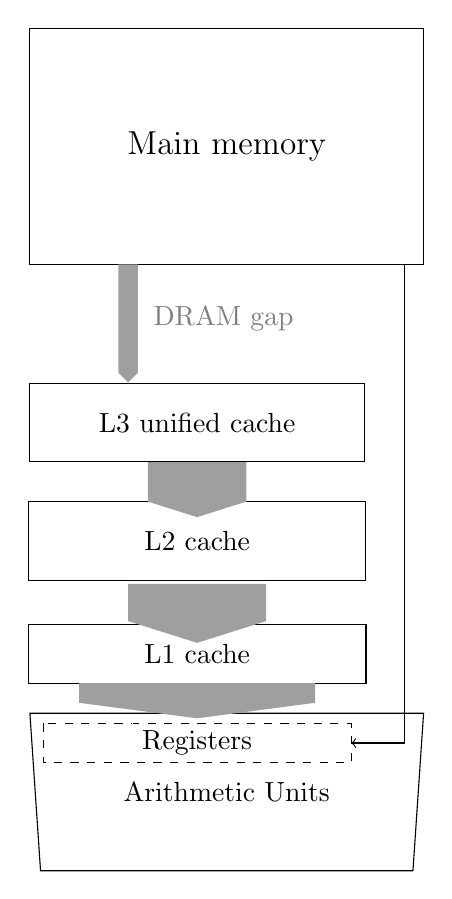
\begin{tikzpicture}
  \draw (0,0) rectangle (5,3) node[fitting node] (RAM) {};
  \node (RAM_label) [draw=white] at(RAM) {\large{}Main memory};
  \node (RAM_right_offset) [coordinate] at($(RAM.south east)!.3!(RAM.south)$) {};
  \node (RAM_left_offset) [coordinate] at($(RAM.south west)!.5!(RAM.south)$) {};

  \node (dram_arrow) [single arrow, rotate=-90, %
  fill=gray!75, minimum height=1.5cm, single arrow head extend=0cm]  at([yshift=-.68cm]RAM_left_offset) {};
  \node (dram_label) [text=gray,right=2mm of dram_arrow.center, anchor=west] {DRAM gap};

  
  \draw ([yshift=-1.5cm]RAM.south west) rectangle ([yshift=-2.5cm]RAM_right_offset) node[fitting node,align=center] (l3cache) {};
  \node (l3cache_label) [draw=white] at(l3cache) {L3 unified cache};
    

  \draw ([yshift=-.5cm]l3cache.south west) rectangle ([yshift=-1.5cm]l3cache.south east) node[fitting node,align=center] (l2cache) {};
  \node (l2cache_label) [draw=white] at(l2cache) {L2 cache};

  % \node (l3_l2_arrow) [single arrow, rotate=-90, %
  % fill=gray!75, minimum width=1.25cm, minimum height=5mm, single arrow head extend=0cm,single arrow tip angle=145 ] at($(l3cache)!.5!(l2cache)$) {};
  \path (l3cache.south) -- (l2cache.north) node[midway, %
  single arrow, %
  rotate=-90, %
  fill=gray!75, %
  minimum width=1.25cm, %
  minimum height=7mm, %
  single arrow head extend=0cm,%
  single arrow tip angle=145] (l3_l2_arrow) {};

  % \node (l2_l1_arrow) [single arrow, rotate=-90, %
  % fill=gray!75, minimum width=1.75cm, minimum height=5mm, single arrow head extend=0cm,single arrow tip angle=145,below right=.1mm of l2cache.south]  {};

      

  \draw ([yshift=-.55cm]l2cache.south west) rectangle ([yshift=-1.3cm]l2cache.south east) node[fitting node] (l1cache) {};
  \node (l1cache_label) [draw=white] at(l1cache) {L1 cache};

    \path (l2cache.south) -- (l1cache.north) node[midway, %
    single arrow, %
    rotate=-90, %
    fill=gray!75, %
    minimum width=1.75cm, %
    minimum height=7.5mm, %
    single arrow head extend=0cm,%
    single arrow tip angle=145] (l2_l1_arrow) {};
  
  
  \draw[dashed,very thin] ($(l1cache.south west)+(.2cm,-.5cm)$) rectangle ($(l1cache.south east)+(-.2cm,-1.cm)$) node[fitting node,align=center] (registers) {};
  


  \node (cpu) [trapezium,draw,minimum width=5cm,minimum height=2cm, trapezium stretches body,rotate=180,below=7.7cm of RAM,anchor=north] {};
  \node (cpu_label) [draw=white] at(cpu) {Arithmetic Units};
  \node (regs_label) [draw=white] at(registers) {Registers};

  \path ($(l1cache.center)!.3!(l1cache.south)$) -- ($(registers.north)$) node[midway, %
    single arrow, %
    rotate=-90, %
    fill=gray!75, %
    minimum width=3cm, %
    minimum height=3.mm, %
    single arrow head extend=0cm,%
    single arrow tip angle=165] (l1_regs_arrow) {};

  \path 
let
\p1
 = ($(RAM.south east)!.1!(RAM.south)$),
\p2
 = (registers.east)
in
coordinate
 (corner_to_registers_east) at (\x1,\y2)
coordinate
 (start_to_registers_east) at (\x1, \y1)
;

\draw[->] (start_to_registers_east) -| (corner_to_registers_east) -- (registers.east);
  \end{tikzpicture}
\end{document}
